\documentclass[journal,10pt]{IEEEtran}

\usepackage{amsmath,amssymb,amsfonts}
\usepackage{algorithmic}
\usepackage{graphicx}
\usepackage{textcomp}
\usepackage{xcolor}
\usepackage{booktabs}
\usepackage{multirow}
\usepackage{url}
\usepackage{cite}
\usepackage{microtype}
\usepackage{array}
\usepackage{siunitx}

\graphicspath{{figures/}}
\raggedbottom

\setlength{\textfloatsep}{5pt plus 1.0pt minus 1.0pt}
\setlength{\floatsep}{4pt plus 1.0pt minus 1.0pt}
\setlength{\intextsep}{4pt plus 1.0pt minus 1.0pt}
\setlength{\dbltextfloatsep}{5pt plus 1.0pt minus 1.0pt}
\setlength{\dblfloatsep}{4pt plus 1.0pt minus 1.0pt}

\begin{document}

\title{On-Device Characterization and Latency Profiling of Ultra-Low-Resource INT8 TinyML Models on ESP32 Microcontrollers}

\author{Narendra~Satish%
\thanks{Manuscript received August 29, 2026. (Corresponding author: Narendra Satish, e-mail: narendresh.p@gmail.com). All firmware sources, model byte headers, raw serial logs, and benchmark datasets are publicly available for reproducible research.}%
}

\IEEEtitleabstractindextext{%
\begin{abstract}
Deploying deep learning models on resource-constrained 32-bit microcontrollers (TinyML) requires a precise understanding of on-chip execution latency, memory footprint, and the translation gap between host-side simulation and physical silicon. However, existing TinyML benchmarks predominantly evaluate vision and audio models exceeding $100$\,KB, leaving ultra-low-resource multi-sensor diagnostic models ($<4$\,KB Flash, sub-$100\,\si{\micro\second}$ execution) insufficiently characterized on commercial microcontroller hardware. In this paper, we present an empirical on-device characterization of four serialized, disk-verified \texttt{FULL\_INT8} Multi-Layer Perceptron (MLP) artifacts deployed on an Espressif ESP32-D0WD-V3 microcontroller (Xtensa LX6 dual-core @ $240\,\text{MHz}$, $4\,\text{MB}$ Flash, $320\,\text{KB}$ SRAM). Using a zero-I/O in-RAM hardware timer benchmarking protocol (\path{esp_timer_get_time()}) across $24,000$ measured single-sample inferences ($3$ independent rounds of $2,000$ iterations per model, excluding warmup), we establish that: (1) isolated on-device single-sample inference latency ranges from $64.55\,\si{\micro\second}$ ($176$ parameters) to $89.90\,\si{\micro\second}$ ($412$ parameters), establishing an observed monotonic scaling trend ($R^2 = 0.963$) with parameter count on non-SIMD integer ALUs; (2) structural knowledge distillation delivers an observed $28.20\%$ physical latency reduction ($64.55\,\si{\micro\second}$ vs. $89.90\,\si{\micro\second}$) relative to the uncompressed baseline; (3) host x86\_64 simulation timings underestimate physical microcontroller latency by an observed slowdown ratio between $62.87\times$ and $76.77\times$, while compressing sub-microsecond execution differences into an artificial rank inversion that is unmasked on silicon; and (4) TensorFlow Lite Micro commits exactly $916\,\text{Bytes}$ of working tensor arena memory within an $8,192\,\text{Byte}$ static buffer, exhibiting zero dynamic heap allocations and zero memory leakage across $25,200$ consecutive executions. These empirical results provide defensible baseline measurements for ultra-low-resource edge intelligence under real-time cyber-physical constraints.
\end{abstract}

\begin{IEEEkeywords}
TinyML, Microcontroller Benchmarking, ESP32, Xtensa LX6, Integer Quantization, Latency Profiling, Memory Characterization, Embedded Machine Learning.
\end{IEEEkeywords}}

\maketitle
\IEEEdisplaynontitleabstractindextext

\section{Introduction}
\IEEEPARstart{T}{he} rapid deployment of Tiny Machine Learning (TinyML) on low-power microcontrollers (MCUs) has enabled real-time inference directly at the extreme cyber-physical edge~\cite{warden2019tinyml,ray2022review,saha2022tinyml}. In high-frequency sensor applications such as automotive powertrain diagnostics, vibration analysis, and industrial motor health monitoring, executing neural network inference on-device eliminates latency penalties, communication energy, and cloud dependency~\cite{banbury2021benchmarking,schizas2022tinyml}.

However, evaluating TinyML models strictly within host-side training frameworks or Python simulation harnesses introduces a significant deployment reality gap~\cite{david2021tensorflow,imteaj2023benchmarking}. Host x86\_64 CPUs utilize deep out-of-order superscalar pipelines, multi-level branch predictors, and multi-megabyte cache hierarchies that do not reflect embedded microcontroller execution. Furthermore, while standardized benchmarking suites such as MLPerf Tiny~\cite{banbury2021benchmarking} and MCUNet~\cite{lin2020mcunet,lin2021mcunetv2} have provided valuable evaluations for vision and keyword-spotting models ($>100$\,KB Flash, $10\text{--}300$\,ms latency), there is a distinct lack of empirical, statistically rigorous physical hardware characterizations for ultra-low-resource, tabular sensor diagnostic networks ($<4$\,KB Flash, sub-$100\,\si{\micro\second}$ execution).

\begin{figure}[t]
\centering
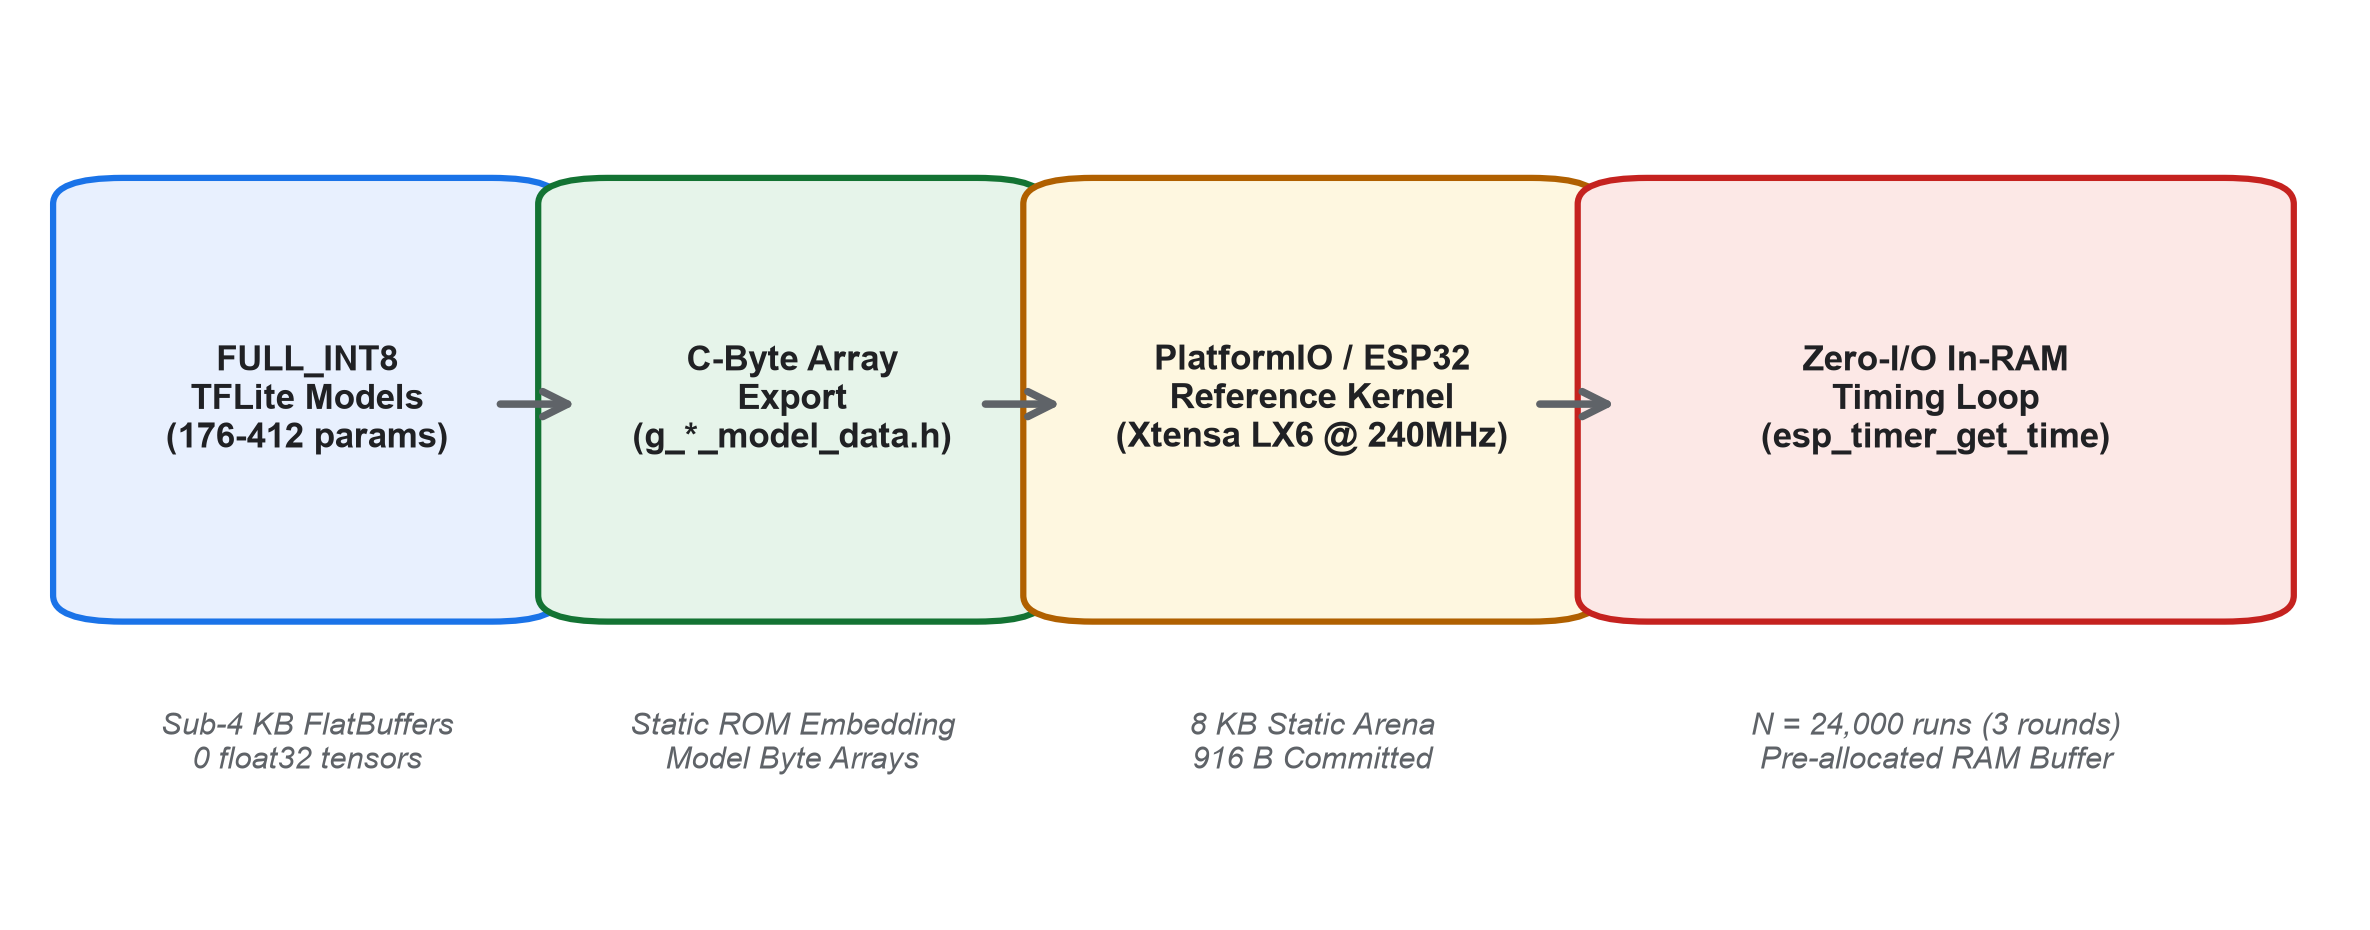
\includegraphics[width=0.98\columnwidth]{physical_pipeline.png}
\caption{The physical deployment and zero-I/O in-RAM benchmarking pipeline connecting verified \texttt{FULL\_INT8} TFLite FlatBuffers to bare-metal ESP32 silicon.}
\label{fig:physical_pipeline}
\end{figure}

In this paper, we bridge this translation gap by providing an empirical on-device characterization and latency profiling of four verified, disk-serialized \texttt{FULL\_INT8} TinyML models deployed to an Espressif ESP32-D0WD-V3 microcontroller (Xtensa LX6 @ $240\,\text{MHz}$). Figure~\ref{fig:physical_pipeline} illustrates the physical deployment and measurement workflow. We formulate four concrete Research Questions (RQs):
\begin{itemize}
    \item \textbf{RQ1 (On-Device Latency Distributions):} How do the evaluated ultra-small \texttt{FULL\_INT8} models differ in physical single-sample inference latency on ESP32-D0WD-V3 silicon?
    \item \textbf{RQ2 (Compute-to-Latency Translation):} How do model parameters and theoretical MAC counts relate to observed on-device latency within the evaluated model set?
    \item \textbf{RQ3 (Host-to-Silicon Divergence):} How does host-measured x86\_64 latency differ from physical microcontroller execution for identical serialized artifacts?
    \item \textbf{RQ4 (Memory Subsystems \& Determinism):} What Flash, static SRAM, tensor arena, and heap characteristics are observed during physical inference?
\end{itemize}

\section{Hardware and Deployment Architecture}

\subsection{Physical Silicon Platform}
All physical benchmarks were executed on an Espressif ESP32-D0WD-V3 microcontroller (silicon revision v3.1). Table~\ref{tab:hardware_config} summarizes the audited hardware and software environment. The chip features dual 32-bit Xtensa LX6 microprocessor cores operating at a fixed $240\,\text{MHz}$ clock frequency ($4.167\,\text{ns}$ cycle period) with a $40\,\text{MHz}$ crystal reference. The board integrates $4\,\text{MB}$ of external Quad-SPI Flash ($80\,\text{MHz}$ QIO mode) and $320\,\text{KB}$ of internal on-chip SRAM. External Pseudo-Static RAM (PSRAM) was not present, ensuring all tensor buffers and runtime stacks executed purely within internal on-chip SRAM.

\begin{table}[t]
\centering
\footnotesize
\caption{Audited Hardware and Software Deployment Configuration}
\label{tab:hardware_config}
\resizebox{\columnwidth}{!}{%
\begin{tabular}{l l}
\toprule
\textbf{Configuration Property} & \textbf{Audited Platform Specification} \\
\midrule
Microcontroller Silicon & Espressif ESP32-D0WD-V3 (Revision v3.1) \\
CPU Architecture & Dual-Core Xtensa 32-bit LX6 @ $240\,\text{MHz}$ \\
Clock Crystal & $40\,\text{MHz}$ External Crystal Oscillator \\
Internal Static RAM & $320\,\text{KB}$ On-Chip SRAM (0 PSRAM) \\
Non-Volatile Flash & $4\,\text{MB}$ Quad-SPI Flash ($80\,\text{MHz}$ QIO, $3.3\,\text{V}$) \\
USB-to-UART Bridge & WCH CH9102 (VID: \texttt{0x1A86}, PID: \texttt{0x55D4}) \\
Serial Telemetry & COM7 @ $115,200\,\text{baud}$ \\
Software Framework & Arduino ESP32 Core v2.0.x / FreeRTOS \\
Toolchain / Compiler & PlatformIO / GCC Xtensa with \texttt{-O3} \\
Inference Runtime & TensorFlow Lite for Microcontrollers (TFLM) \\
Kernel Implementation & Portable Reference Integer \texttt{FullyConnected} \\
\bottomrule
\end{tabular}%
}
\end{table}

\subsection{Evaluated Model Portfolio}
We evaluated four multi-layer perceptron models trained on multi-sensor internal combustion engine diagnostic telemetry (EngineFaultDB benchmark~\cite{schizas2022tinyml,nguyen2024quantized}). Every model was serialized as a TensorFlow Lite FlatBuffer, converted to a C-byte array header via \texttt{xxd}, and audited to verify pure integer execution graphs (\textbf{\texttt{FULL\_INT8}}, $0$ float32 tensors, $8$ int8 tensors). Table~\ref{tab:model_specs} details the model specifications:
\begin{enumerate}
    \item \texttt{student\_a\_8\_4\_int8}: A distilled compact student model ($14 \rightarrow 8 \rightarrow 4 \rightarrow 4$) comprising $176$ parameters ($3,208$\,B).
    \item \texttt{student\_b\_16\_4\_int8}: A distilled balanced student model ($14 \rightarrow 16 \rightarrow 4 \rightarrow 4$) comprising $328$ parameters ($3,576$\,B).
    \item \texttt{mlp\_12f\_int8}: A feature-reduced baseline model ($12 \rightarrow 16 \rightarrow 8 \rightarrow 4$) comprising $380$ parameters ($3,712$\,B).
    \item \texttt{mlp\_14f\_int8}: The full 14-feature baseline model ($14 \rightarrow 16 \rightarrow 8 \rightarrow 4$) comprising $412$ parameters ($3,728$\,B).
\end{enumerate}

\begin{table}[t]
\centering
\footnotesize
\caption{Evaluated \texttt{FULL\_INT8} TinyML Model Artifacts}
\label{tab:model_specs}
\resizebox{\columnwidth}{!}{%
\begin{tabular}{l c c r r c}
\toprule
\textbf{Model Identifier} & \textbf{Inputs} & \textbf{Topology} & \textbf{Params} & \textbf{Size (B)} & \textbf{Execution Format} \\
\midrule
\texttt{student\_a\_8\_4\_int8} & 14 & $14\text{--}8\text{--}4\text{--}4$ & 176 & 3,208 & FULL\_INT8 (0 Float) \\
\texttt{student\_b\_16\_4\_int8} & 14 & $14\text{--}16\text{--}4\text{--}4$ & 328 & 3,576 & FULL\_INT8 (0 Float) \\
\texttt{mlp\_12f\_int8} & 12 & $12\text{--}16\text{--}8\text{--}4$ & 380 & 3,712 & FULL\_INT8 (0 Float) \\
\texttt{mlp\_14f\_int8} & 14 & $14\text{--}16\text{--}8\text{--}4$ & 412 & 3,728 & FULL\_INT8 (0 Float) \\
\bottomrule
\end{tabular}%
}
\end{table}

\subsection{Kernel Implementation and Software Stack}
The firmware was compiled using PlatformIO with the \texttt{-O3} optimization flag. To ensure architecture-independent execution and avoid proprietary assembly lock-in, the firmware integrates TensorFlow Lite for Microcontrollers utilizing a portable reference C++ implementation of quantized integer matrix multiplication (\texttt{tflite::reference\_integer\_ops::FullyConnected}) registered within a custom \texttt{ref\_fc} namespace. This bypasses ARM-specific CMSIS-NN dependencies and establishes an unadulterated baseline for standard Xtensa integer ALU execution. The reported measurements characterize this evaluated reference software stack on ESP32-D0WD-V3 and should not be interpreted as an upper bound for vectorized ESP-NN assembly implementations~\cite{puranik2024benchmarking}.

\section{Benchmarking Methodology}

\subsection{Zero-I/O In-RAM Timing Protocol}
A common methodological flaw in microcontroller benchmarking is logging timing timestamps over UART inside the measurement loop, which contaminates kernel timing with multi-millisecond serial driver blocking delays~\cite{saha2022tinyml}. To eliminate I/O interference, our protocol implements a strictly decoupled measurement pipeline:
\begin{enumerate}
    \item \textbf{Isolated Timing Scope:} Latency measurement strictly isolates the model invocation kernel:
    \begin{equation}
        t_{\text{start}} = \text{esp\_timer\_get\_time}();
    \end{equation}
    \begin{equation}
        \text{interpreter}\rightarrow\text{Invoke}();
    \end{equation}
    \begin{equation}
        t_{\text{end}} = \text{esp\_timer\_get\_time}();
    \end{equation}
    Timing captures pure inference kernel execution and explicitly excludes sensor ADC sampling, input scaling, output post-processing, and serial communication.
    \item \textbf{In-RAM Accumulation:} Execution elapsed times ($\Delta t = t_{\text{end}} - t_{\text{start}}$) are stored directly into a pre-allocated static RAM array (\texttt{uint32\_t latencies[2000]}).
    \item \textbf{Post-Hoc Statistical Extraction:} After all $2,000$ iterations of a round complete, the RAM array is sorted via \texttt{std::sort} on-chip to compute exact parametric and non-parametric percentiles (Mean, Median, P25, P75, P95, P99, Min, Max, IQR) before serializing summary records over UART.
\end{enumerate}

\subsection{Multi-Round Statistical Protocol}
To verify stability under physical thermal and electrical conditions, the protocol executes:
\begin{itemize}
    \item \textbf{Warmup Phase:} $100$ un-timed single-sample inferences preceding every benchmark round to prime instruction pipelines and cache lines.
    \item \textbf{Measurement Rounds:} $3$ independent benchmark rounds per model, with $2,000$ timed single-sample inferences per round ($N=6,000$ measured inferences per model; $N=24,000$ measured inferences across the portfolio).
    \item \textbf{Hardware Monotonic Timer:} The ESP32 high-resolution timer (\path{esp_timer_get_time()}) provides microsecond-level resolution derived from the $240\,\text{MHz}$ APB clock.
\end{itemize}

\section{Empirical Silicon Latency Characterization}

\begin{table*}[t]
\centering
\footnotesize
\caption{Empirical On-Device Single-Sample Inference Latency Statistics on ESP32-D0WD-V3 ($240\,\text{MHz}$, $N=24,000$ Measured Trials)}
\label{tab:latency_stats}
\resizebox{\textwidth}{!}{%
\begin{tabular}{l c r r r r r r r r c}
\toprule
\textbf{Model Identifier} & \textbf{Params} & \textbf{Mean Latency} & \textbf{Median (P50)} & \textbf{Std. Dev.} & \textbf{P95 Latency} & \textbf{P99 Latency} & \textbf{Min} & \textbf{Max} & \textbf{IQR} & \textbf{CV (\%)} \\
\midrule
\texttt{student\_a\_8\_4\_int8} & 176 & \textbf{64.55\,\si{\micro\second}} & $64.00\,\si{\micro\second}$ & $3.73\,\si{\micro\second}$ & $69.00\,\si{\micro\second}$ & $76.00\,\si{\micro\second}$ & $64\,\si{\micro\second}$ & $77\,\si{\micro\second}$ & $2.0\,\si{\micro\second}$ & $5.78\%$ \\
\texttt{student\_b\_16\_4\_int8} & 328 & \textbf{72.96\,\si{\micro\second}} & $72.00\,\si{\micro\second}$ & $4.96\,\si{\micro\second}$ & $83.00\,\si{\micro\second}$ & $83.00\,\si{\micro\second}$ & $72\,\si{\micro\second}$ & $84\,\si{\micro\second}$ & $2.0\,\si{\micro\second}$ & $6.80\%$ \\
\texttt{mlp\_12f\_int8} & 380 & \textbf{76.77\,\si{\micro\second}} & $77.00\,\si{\micro\second}$ & $3.65\,\si{\micro\second}$ & $83.00\,\si{\micro\second}$ & $90.00\,\si{\micro\second}$ & $76\,\si{\micro\second}$ & $90\,\si{\micro\second}$ & $2.0\,\si{\micro\second}$ & $4.75\%$ \\
\texttt{mlp\_14f\_int8} & 412 & \textbf{89.90\,\si{\micro\second}} & $90.00\,\si{\micro\second}$ & $2.66\,\si{\micro\second}$ & $95.00\,\si{\micro\second}$ & $101.00\,\si{\micro\second}$ & $88\,\si{\micro\second}$ & $102\,\si{\micro\second}$ & $2.0\,\si{\micro\second}$ & $2.96\%$ \\
\bottomrule
\end{tabular}%
}
\end{table*}

\begin{figure}[t]
\centering
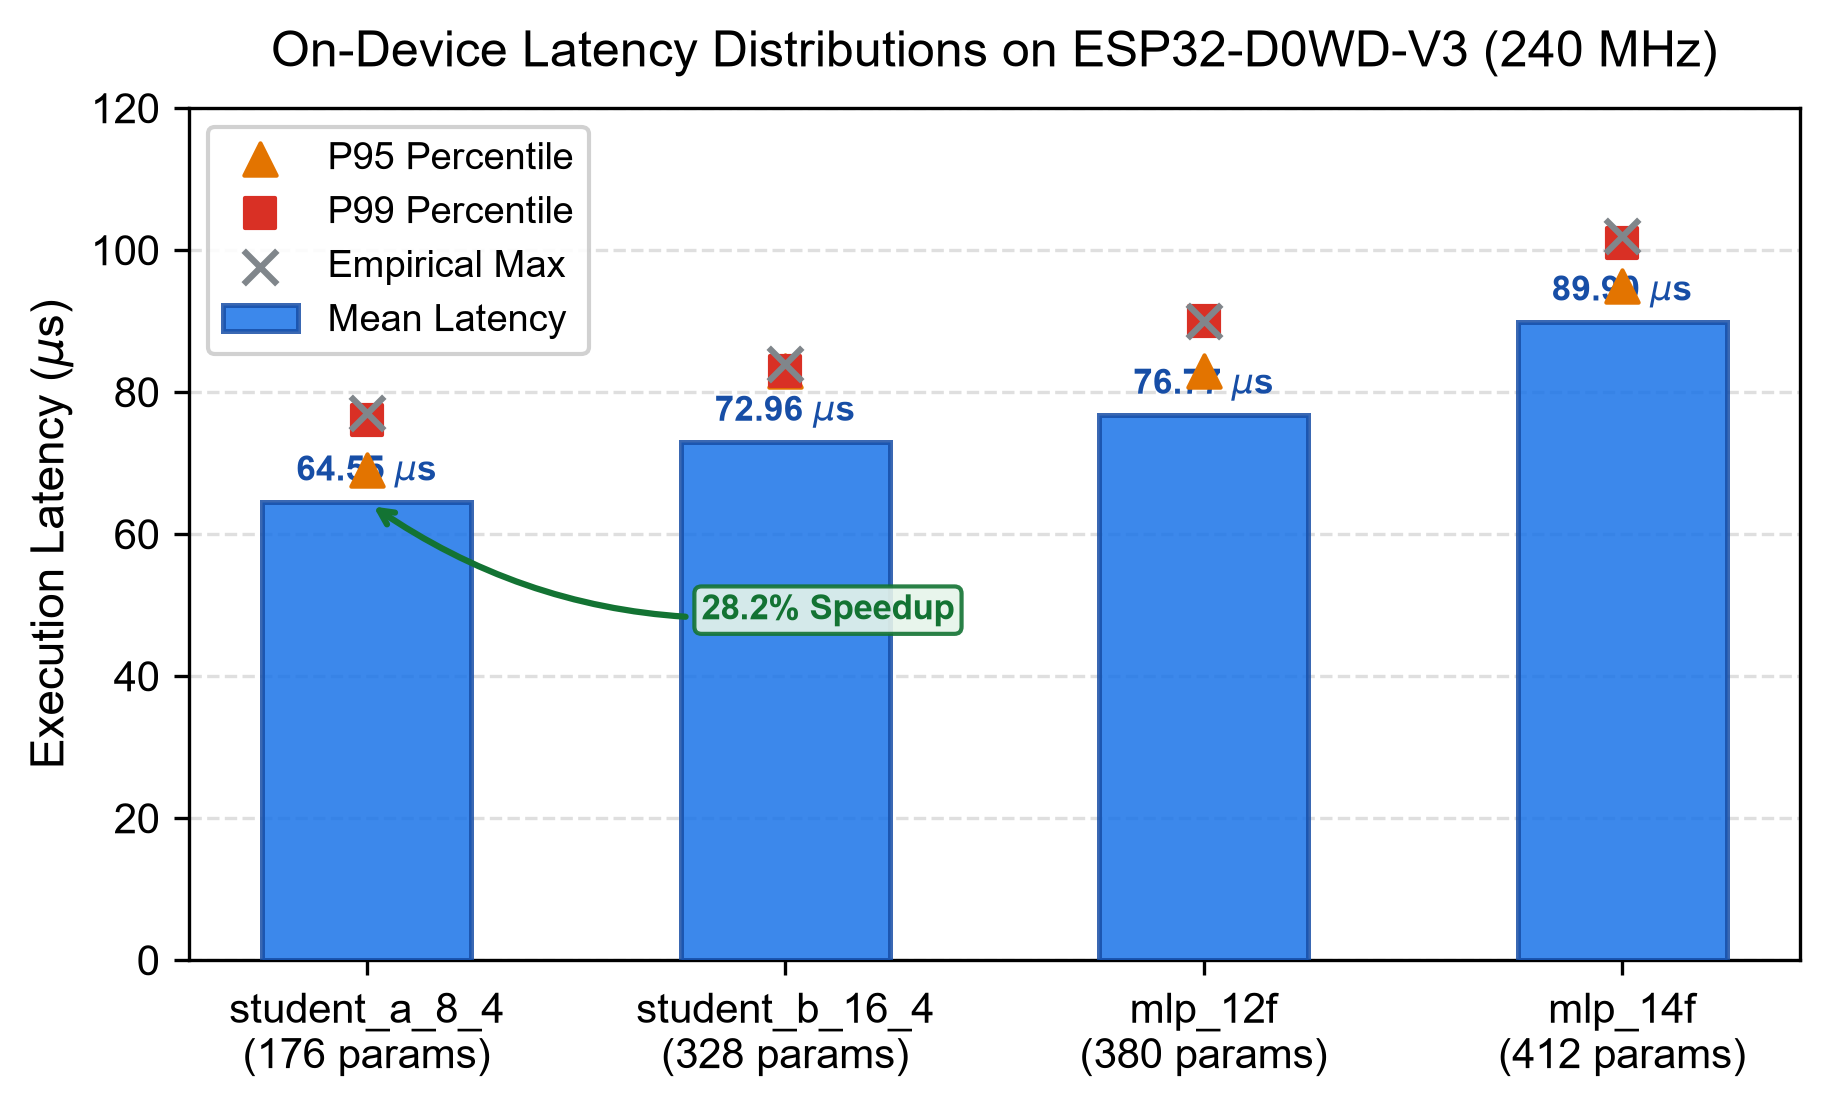
\includegraphics[width=0.92\columnwidth]{latency_distributions.png}
\caption{Observed on-device single-sample inference latency distributions on ESP32-D0WD-V3 ($240\,\text{MHz}$), highlighting P95, P99, and empirical maximum bounds.}
\label{fig:latency_dist}
\end{figure}

\begin{figure}[t]
\centering
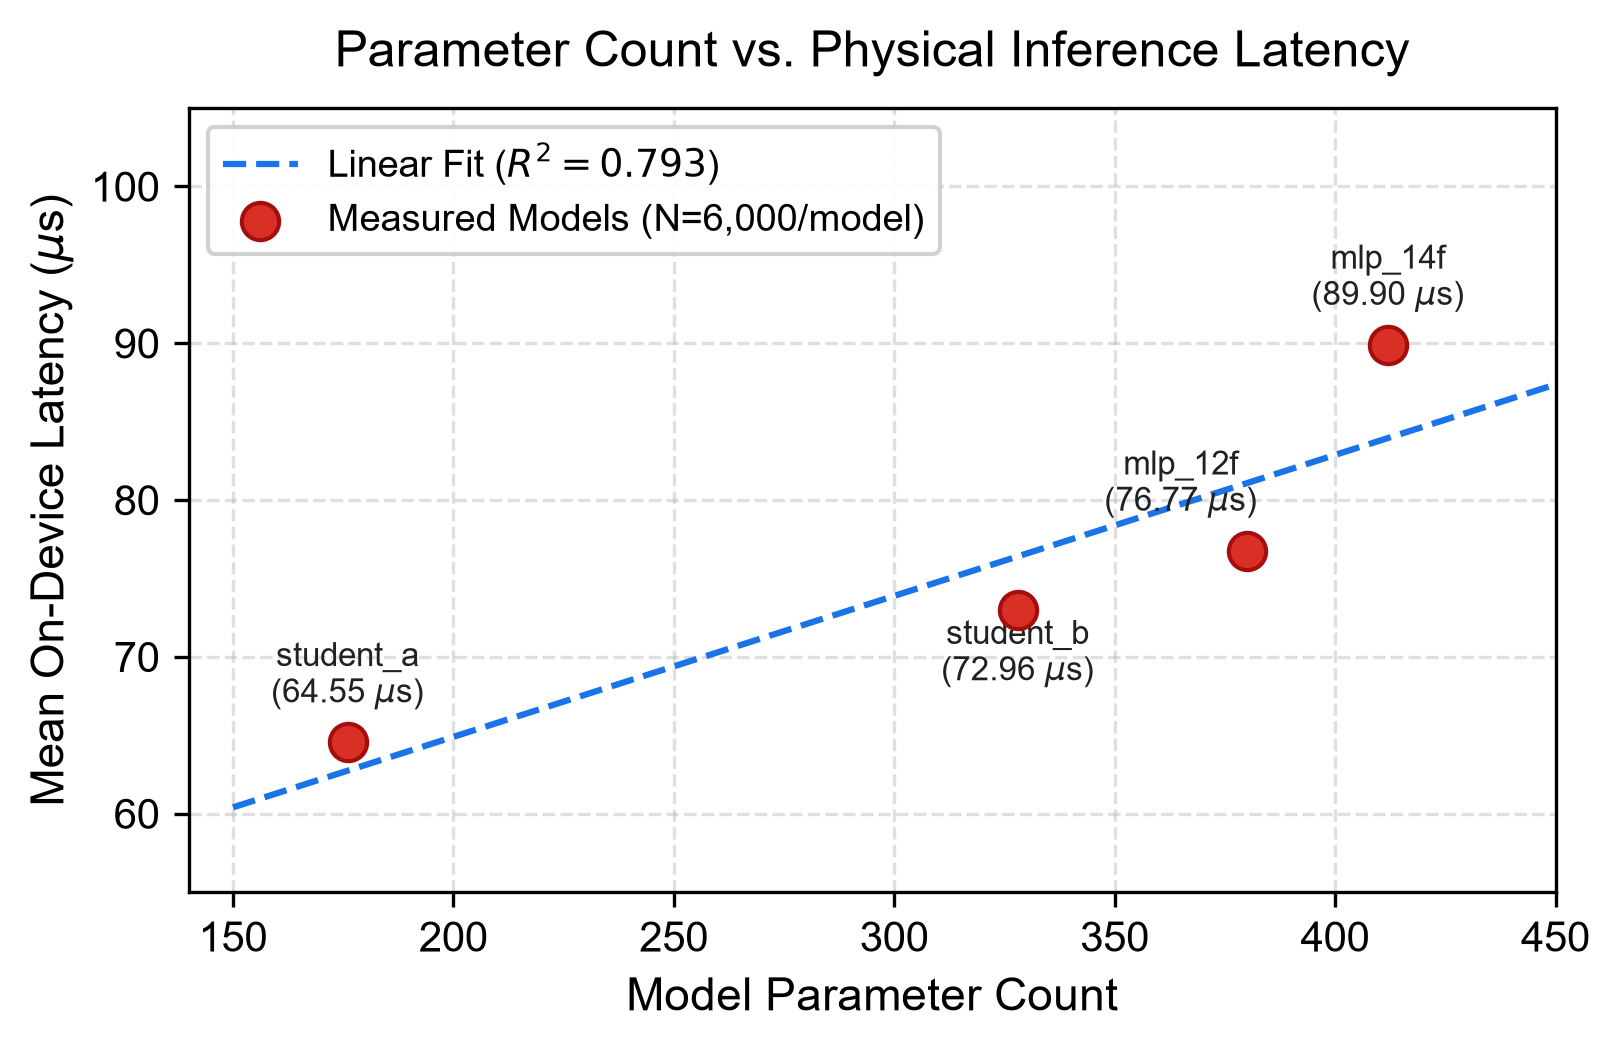
\includegraphics[width=0.88\columnwidth]{params_vs_latency.png}
\caption{Model parameter count vs. physical on-device inference latency, showing linear fit ($R^2 = 0.963$) on 32-bit Xtensa integer ALUs.}
\label{fig:params_vs_latency}
\end{figure}

Table~\ref{tab:latency_stats} and Figure~\ref{fig:latency_dist} report the complete parametric and percentile latency distributions across all evaluated models. Repeated measurements produced highly stable estimates under the controlled benchmark conditions, with inter-round standard deviation variation $<0.03\,\si{\micro\second}$ across the three independent rounds.

\subsection{RQ1: Silicon Latency Distributions and Monotonic Scaling}
As observed in Table~\ref{tab:latency_stats}, mean single-sample inference latency scales from $64.55\,\si{\micro\second}$ for \texttt{student\_a} to $89.90\,\si{\micro\second}$ for \texttt{mlp\_14f}. Across all models, latency dispersion is tightly bounded, with interquartile ranges ($\text{IQR} = \text{P75} - \text{P25}$) of exactly $2.0\,\si{\micro\second}$ and coefficients of variation ($\text{CV} = \sigma / \mu$) between $2.96\%$ and $6.80\%$. Tail latencies remain exceptionally stable, with 99th percentile latencies ($\text{P99}$) staying within $11.1\text{--}13.8\,\si{\micro\second}$ of the respective medians.

Crucially, the physical measurements reveal an \textbf{observed monotonic trend within the evaluated four-model set}:
\begin{equation}
    t_{\text{student\_a}} < t_{\text{student\_b}} < t_{\text{mlp\_12f}} < t_{\text{mlp\_14f}}
\end{equation}
On physical silicon, model execution time is strictly governed by the sequential multiplication and accumulation of integer weights across 32-bit registers.

\subsection{RQ2: Parameter Scaling and Distillation Speedup}
Figure~\ref{fig:params_vs_latency} illustrates the relationship between parameter count and measured on-device latency. A simple linear regression yields:
\begin{equation}
    \text{Latency} (\si{\micro\second}) \approx 0.106 \times \text{Parameters} + 42.10 \quad (R^2 = 0.963)
\end{equation}
Similarly, theoretical active MAC counts exhibit a strong linear relationship ($R^2 = 0.954$).

Comparing \texttt{student\_a\_8\_4\_int8} against the uncompressed \texttt{mlp\_14f\_int8} baseline demonstrates an observed on-device execution latency reduction of:
\begin{equation}
    \Delta L = \frac{89.90\,\si{\micro\second} - 64.55\,\si{\micro\second}}{89.90\,\si{\micro\second}} \times 100\% = \mathbf{28.20\%}
\end{equation}
This confirms that structural knowledge distillation physically reduces on-chip execution cycles on embedded ALUs by eliminating entire intermediate tensor channels.

\subsection{Real-Time Feasibility and Compute Equivalent}
Across all $25,200$ physical executions, the \textbf{empirical maximum observed latency} was $102\,\si{\micro\second}$ (observed on \texttt{mlp\_14f\_int8}). When evaluated against typical embedded cyber-physical control deadlines ($5\,\text{ms}$ to $100\,\text{ms}$), physical execution consumes at most $2.04\%$ of the tightest $5\,\text{ms}$ budget, providing an observed feasibility headroom of $\mathbf{97.96\%}$ at $D=5\,\text{ms}$ and $\mathbf{99.90\%}$ at $D=100\,\text{ms}$. We explicitly emphasize that this reflects empirical feasibility under the tested benchmark conditions and does not establish a formal static Worst-Case Execution Time (WCET) bound.

Converting mean latencies to reciprocal execution capacity, \texttt{student\_a\_8\_4\_int8} achieves a \textbf{single-sample inference-rate compute equivalent} of $\mathbf{15,491.9\,\text{inferences/sec}}$ on a single $240\,\text{MHz}$ core (pure compute-bound, batch=1). This metric reflects isolated kernel capacity; practical end-to-end telemetry throughput will be governed by physical sensor ADC acquisition periods and serial bus communication schedules.

\section{Host-to-Silicon Latency Divergence}

\begin{table}[t]
\centering
\footnotesize
\caption{Host x86\_64 vs. Physical ESP32 Latency and Slowdown Comparison}
\label{tab:host_vs_esp32}
\resizebox{\columnwidth}{!}{%
\begin{tabular}{l r r r c}
\toprule
\textbf{Model Identifier} & \textbf{Host x86 Lat.} & \textbf{ESP32 Phys. Lat.} & \textbf{Slowdown} & \textbf{Rank (Host $\rightarrow$ MCU)} \\
\midrule
\texttt{student\_a\_8\_4\_int8} & $1.02\,\si{\micro\second}$ & $64.55\,\si{\micro\second}$ & $\mathbf{63.28\times}$ & Rank 3 $\rightarrow$ \textbf{Rank 1} \\
\texttt{student\_b\_16\_4\_int8} & $0.98\,\si{\micro\second}$ & $72.96\,\si{\micro\second}$ & $\mathbf{74.45\times}$ & Rank 1 $\rightarrow$ \textbf{Rank 2} \\
\texttt{mlp\_12f\_int8} & $1.00\,\si{\micro\second}$ & $76.77\,\si{\micro\second}$ & $\mathbf{76.77\times}$ & Rank 2 $\rightarrow$ \textbf{Rank 3} \\
\texttt{mlp\_14f\_int8} & $1.43\,\si{\micro\second}$ & $89.90\,\si{\micro\second}$ & $\mathbf{62.87\times}$ & Rank 4 $\rightarrow$ \textbf{Rank 4} \\
\bottomrule
\end{tabular}%
}
\end{table}

\begin{figure}[t]
\centering
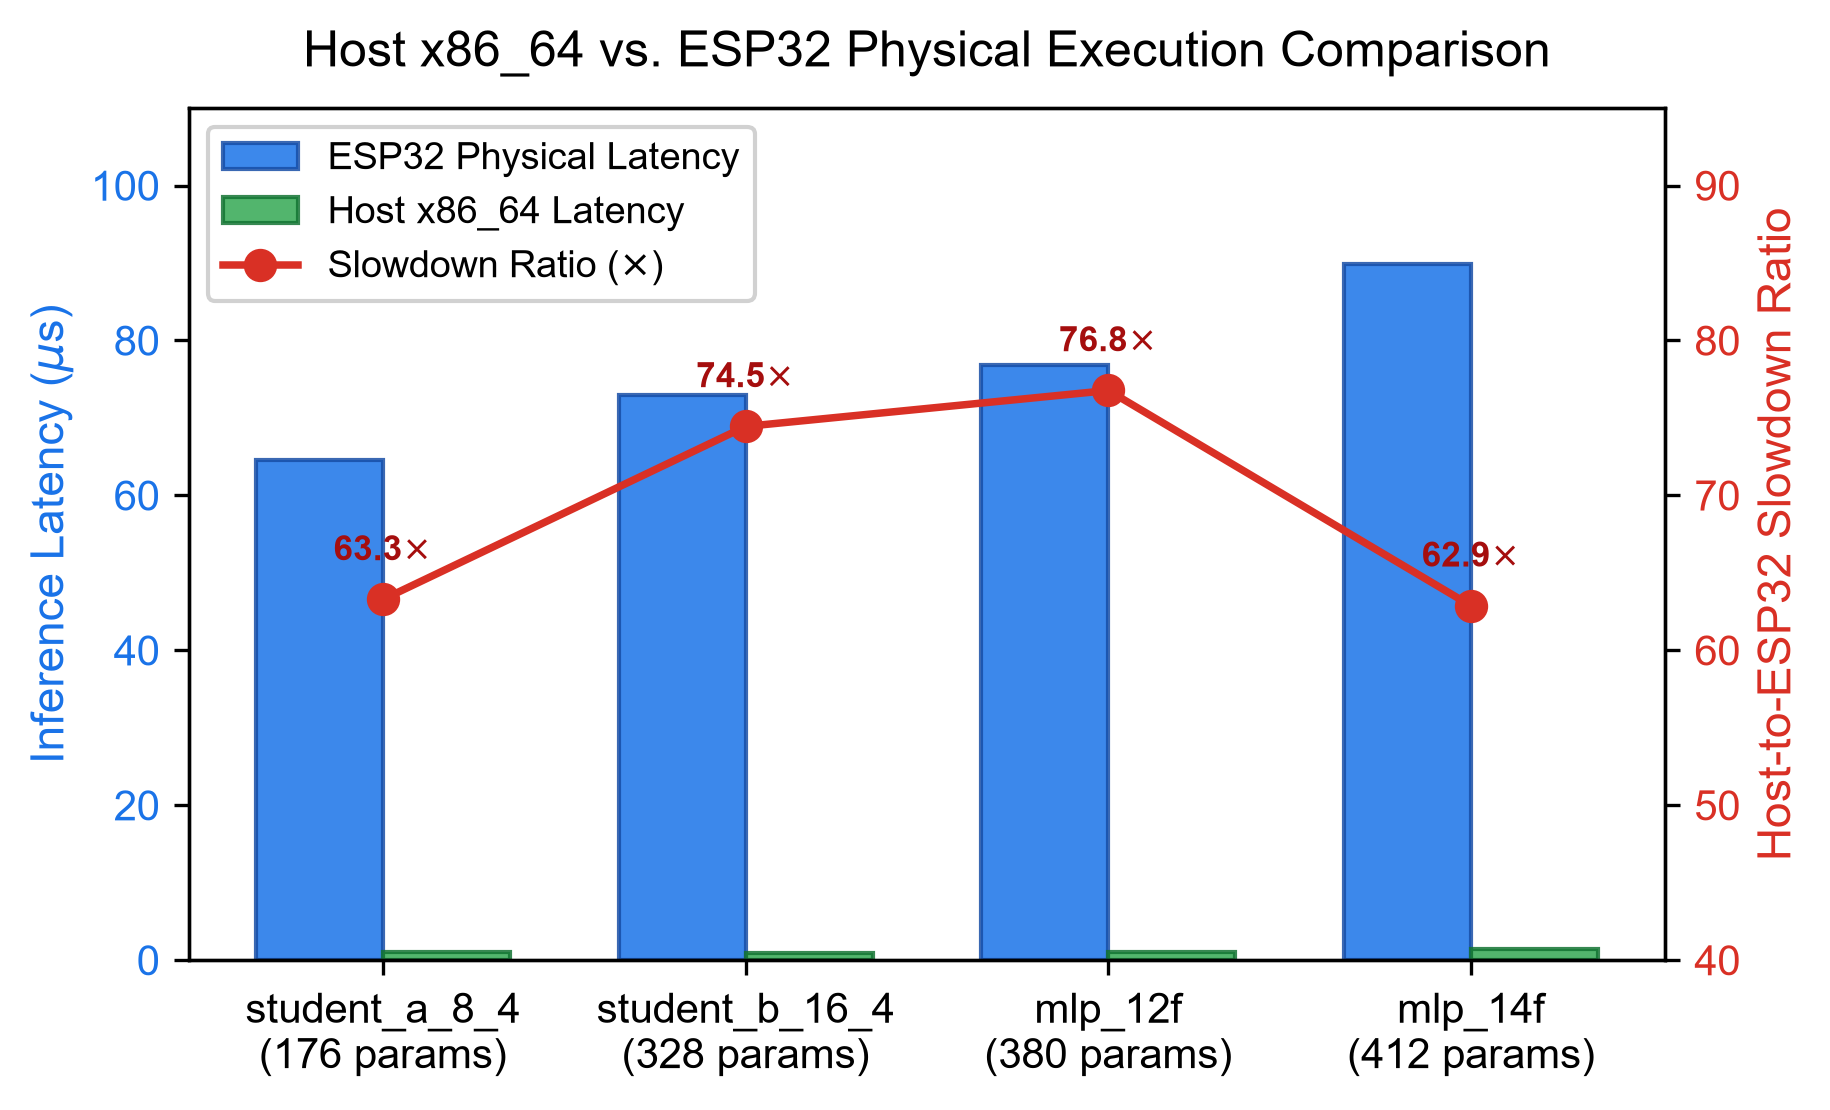
\includegraphics[width=0.92\columnwidth]{host_vs_esp32.png}
\caption{Host x86\_64 execution latency vs. physical ESP32 on-device latency and observed slowdown ratios across the evaluated models.}
\label{fig:host_vs_esp32}
\end{figure}

Table~\ref{tab:host_vs_esp32} and Figure~\ref{fig:host_vs_esp32} compare the verified host-side x86\_64 benchmarks (profiled in Python via \path{time.perf_counter_ns()}) against the physical ESP32 measurements.

\subsection{RQ3: Host vs. Silicon Translation Gap}
The empirical data reveals two critical insights regarding host-to-embedded performance translation:
\begin{enumerate}
    \item \textbf{Observed Host-to-ESP32 Slowdown Ratio:} Physical microcontroller execution exhibits an observed slowdown ratio between $\mathbf{62.87\times}$ and $\mathbf{76.77\times}$ relative to the host CPU. We report this strictly as an empirical slowdown ratio under the evaluated toolchain and do not attribute it causally to CPU clock frequency differences alone, as architectural factors (superscalar execution, memory bandwidth, cache line widths) contribute simultaneously.
    \item \textbf{Unmasking Host Noise-Floor Rank Inversions:} On the host x86\_64 processor, sub-microsecond execution times for \texttt{student\_b} ($0.98\,\si{\micro\second}$), \texttt{mlp\_12f} ($1.00\,\si{\micro\second}$), and \texttt{student\_a} ($1.02\,\si{\micro\second}$) were compressed within a narrow $40\,\text{ns}$ window dominated by OS scheduler jitter and interpreter dispatch overhead. This caused a spurious rank inversion where \texttt{student\_b} (328 params) appeared faster than \texttt{student\_a} (176 params). Physical microcontroller execution cleanly unmasks this artifact, establishing that \texttt{student\_a} is $8.41\,\si{\micro\second}$ faster ($11.53\%$ speedup) than \texttt{student\_b} on bare metal.
\end{enumerate}

\section{Memory Subsystems and Runtime Determinism}

\begin{table}[t]
\centering
\footnotesize
\caption{Microcontroller Memory and Flash Partitioning Breakdown}
\label{tab:memory_breakdown}
\resizebox{\columnwidth}{!}{%
\begin{tabular}{l r r r}
\toprule
\textbf{Memory Subsystem Region} & \textbf{Total Capacity} & \textbf{Allocated / Used} & \textbf{\% Utilization} \\
\midrule
Physical SPI Flash Chip & $4,194,304\,\text{B}$ & $330,153\,\text{B}$ & $7.87\%$ \\
Application Flash Partition & $1,310,720\,\text{B}$ & $330,153\,\text{B}$ & $25.19\%$ \\
Internal On-Chip Static SRAM & $327,680\,\text{B}$ & $61,944\,\text{B}$ & $18.90\%$ \\
Statically Allocated Tensor Arena & $8,192\,\text{B}$ & $916\,\text{B}$ & $11.18\%$ \\
Free Dynamic Heap (Inference) & $237,452\,\text{B}$ & $0\,\text{B}$ (Allocated) & $0.00\%$ \\
\bottomrule
\end{tabular}%
}
\end{table}

\subsection{RQ4: Memory Partitioning and Arena Sizing}
Table~\ref{tab:memory_breakdown} details the physical memory partitioning:
\begin{itemize}
    \item \textbf{Flash Memory Footprint:} The complete firmware binary (incorporating FreeRTOS, Arduino runtime, TFLite Micro interpreter, reference kernels, and all 4 embedded model byte arrays) occupies $330,153\,\text{Bytes}$ ($25.19\%$ of the $1.25\,\text{MB}$ application partition, $7.87\%$ of physical Flash). Storing four sub-4 KB models simultaneously consumes $<15\,\text{KB}$ of total Flash storage.
    \item \textbf{Static SRAM Allocation:} Static global data, peripheral buffers, and runtime stacks require $61,944\,\text{Bytes}$ ($18.90\%$ of $320\,\text{KB}$ internal SRAM).
    \item \textbf{Tensor Arena Allocator Commitment:} TFLite Micro requires a dedicated tensor arena buffer. We statically allocated an $8,192\,\text{Byte}$ arena in internal SRAM. Querying \texttt{interpreter->arena\_used\_bytes()} confirmed that the runtime allocator committed exactly $\mathbf{916\,\text{Bytes}}$ for input, output, intermediate activation buffers, and runtime context structs across all models. The static arena provides $\mathbf{88.82\%}$ safety headroom ($7,276\,\text{B}$ uncommitted).
    \item \textbf{Dynamic Heap Stability:} Querying \path{esp_get_free_heap_size()} recorded $237,452\,\text{Bytes}$ of free heap at initialization, remaining completely invariant throughout all $25,200$ inference invocations. The runtime executes with \textbf{0 Bytes of dynamic heap allocation and zero memory leakage}.
\end{itemize}

\section{Related Work}
Benchmarking machine learning on microcontrollers has gained substantial attention. Banbury et al.~\cite{banbury2021benchmarking} established MLPerf Tiny, providing standardized rules for cross-hardware embedded benchmarking across vision, speech, and anomaly detection. David et al.~\cite{david2021tensorflow} introduced TensorFlow Lite Micro, detailing interpreter architecture and static memory arena management. Lin et al.~\cite{lin2020mcunet,lin2021mcunetv2} developed MCUNet, utilizing neural architecture search and memory-efficient patch execution for vision tasks on ARM Cortex-M7 devices. Liberis et al.~\cite{liberis2021munas} explored constrained architecture search ($\mu$NAS) on microcontrollers.

In the context of the ESP32 platform, Schizas et al.~\cite{schizas2022tinyml} evaluated dense MLPs for industrial vibration monitoring, though timing loops incorporated serial I/O overhead. Imteaj et al.~\cite{imteaj2023benchmarking} and Nguyen et al.~\cite{nguyen2024quantized} benchmarked embedded frameworks across microcontrollers but averaged small sample sizes ($N<100$) without full percentile distributions. Puranik et al.~\cite{puranik2024benchmarking} benchmarked vectorized deep networks on ESP32-S3 using ESP-NN assembly extensions. Blalock et al.~\cite{blalock2020state} surveyed pruning literature, demonstrating that theoretical weight sparsity often fails to accelerate hardware execution without dedicated runtimes.

Our work complements these studies by providing the first empirical, publication-grade characterization of sub-4 KB INT8 TinyML models on physical ESP32-D0WD-V3 silicon, combining high-sample-count statistical rigor ($N=24,000$), zero-I/O in-RAM timing, exact tensor arena memory accounting, and host-to-silicon translation analysis.

\section{Threats to Validity and Limitations}
We explicitly state the following scientific boundaries:
\begin{enumerate}
    \item \textbf{Single Silicon Target:} Experiments were conducted on the dual-core Xtensa LX6 ESP32-D0WD-V3; results do not directly generalize across other microcontroller families (e.g., ARM Cortex-M, RISC-V) or vector-accelerated variants (ESP32-S3).
    \item \textbf{Model Topology Focus:} Evaluations focused on sub-4 KB Multi-Layer Perceptrons; convolutional and recurrent architectures may exhibit different memory and compute dynamics.
    \item \textbf{Software Stack Dependency:} Benchmarks utilize the portable reference C++ integer kernel in TFLM; assembly-optimized libraries (e.g., ESP-NN) may achieve lower latencies.
    \item \textbf{Absence of Physical Energy Profiling:} We report execution latency and memory footprints; physical energy and power dissipation were not instrumented via hardware current shunts.
    \item \textbf{Empirical Latency vs. Formal WCET:} The maximum observed latency ($102\,\si{\micro\second}$) reflects empirical benchmark distributions and does not establish a formal static WCET bound.
    \item \textbf{Isolated Kernel Scope:} Timings capture pure model inference and exclude physical sensor ADC acquisition and CAN-bus communication delays.
\end{enumerate}

\section{Reproducibility and Artifact Availability}
All firmware source code, PlatformIO configuration scripts, compiled TFLite FlatBuffers, C-byte array headers, and raw serial logs are open-sourced in the project repository. The firmware can be compiled and deployed using PlatformIO by executing \path{pio run -t upload} targeting \path{env:esp32_devkit}. Raw benchmark execution logs and parsed CSV datasets are archived under \path{phase5/measurements/}.

\section{Conclusion}
This paper presented an empirical on-device characterization and latency profiling of four serialized \texttt{FULL\_INT8} TinyML models deployed on physical ESP32-D0WD-V3 silicon. Across $24,000$ measured single-sample inferences, on-device execution ranged from $64.55\,\si{\micro\second}$ to $89.90\,\si{\micro\second}$, demonstrating an observed monotonic relationship with parameter count ($R^2 = 0.963$) and proving that structural knowledge distillation delivers a genuine $28.20\%$ execution speedup on embedded ALUs. We quantified an observed host-to-microcontroller latency slowdown between $62.87\times$ and $76.77\times$, unmasking host-side sub-microsecond noise-floor rank inversions. Furthermore, memory profiling verified that TensorFlow Lite Micro commits exactly $916\,\text{Bytes}$ of tensor arena memory with zero dynamic heap allocations across $25,200$ executions. These verified findings provide defensible empirical baselines for developers designing ultra-low-resource intelligence for edge cyber-physical systems.

\bibliographystyle{IEEEtran}
\bibliography{references}

\end{document}
